\chapter{Pengenalan Unsupervised Learning}

\section{Pengantar Unsupervised Learning}

\textbf{Unsupervised Learning} merupakan salah satu pendekatan utama dalam Machine Learning yang digunakan ketika data yang tersedia tidak memiliki label atau keluaran yang diketahui sebelumnya. Berbeda dengan \textit{supervised learning}, di mana model dilatih berdasarkan pasangan data input dan output, dalam \textit{unsupervised learning} model berusaha menemukan struktur, pola, atau keteraturan tersembunyi di dalam data secara mandiri tanpa panduan eksplisit \cite{hastie2009elements}.

Tujuan utama dari unsupervised learning bukanlah membuat prediksi terhadap label yang telah ditentukan, melainkan mengekstraksi representasi yang bermanfaat, melakukan segmentasi, atau mereduksi kompleksitas data agar lebih mudah dipahami dan dianalisis. Dalam konteks bisnis, pendekatan ini sangat berguna ketika organisasi memiliki banyak data historis tetapi tidak memiliki anotasi atau hasil akhir yang terstruktur secara eksplisit.

Contoh nyata dari penerapan unsupervised learning dalam dunia bisnis meliputi:
\begin{itemize}
	\item \textbf{Segmentasi pelanggan:} mengelompokkan pelanggan ke dalam segmen-segmen homogen berdasarkan perilaku pembelian, preferensi, atau demografi tanpa perlu label manual.
	\item \textbf{Deteksi anomali:} mengidentifikasi transaksi yang tidak biasa atau mencurigakan dalam sistem keuangan tanpa memerlukan contoh eksplisit dari penipuan sebelumnya.
	\item \textbf{Reduksi dimensi:} menyederhanakan data berdimensi tinggi (seperti data sensor IoT atau profil pelanggan) untuk memudahkan visualisasi dan analisis lebih lanjut.
\end{itemize}

Salah satu perbedaan mendasar antara supervised dan unsupervised learning adalah \textbf{ketersediaan label}. Pada supervised learning, model didorong untuk belajar dari hubungan antara input dan output yang telah diketahui, sedangkan pada unsupervised learning, tidak ada target output yang eksplisit. Oleh karena itu, evaluasi keberhasilan model unsupervised sering kali memerlukan pendekatan eksploratif, visualisasi, atau validasi eksternal berbasis domain bisnis.

Secara umum, unsupervised learning sangat cocok digunakan pada tahap eksplorasi awal dalam proses analitik data, terutama ketika:
\begin{itemize}
	\item Label data sulit diperoleh atau membutuhkan biaya tinggi,
	\item Tujuan analisis bersifat eksploratif, misalnya memahami struktur data,
	\item Organisasi ingin menggali pola baru atau potensi segmen yang belum diketahui.
\end{itemize}

Pendekatan ini sangat relevan dalam era Big Data, di mana data yang tersedia terus bertambah tetapi tidak selalu teranotasi secara manual. Unsupervised learning memungkinkan organisasi untuk memperoleh wawasan awal yang penting, mengelompokkan entitas yang serupa, dan mengenali outlier yang berpotensi mengindikasikan risiko atau peluang tersembunyi \cite{ghahramani2004unsupervised}.

Dengan memahami prinsip dasar unsupervised learning, pengambil keputusan dapat lebih siap untuk mengidentifikasi area bisnis yang dapat memperoleh manfaat dari segmentasi otomatis, deteksi pola tersembunyi, dan eksplorasi data yang lebih dalam sebagai landasan untuk strategi berbasis data.

\section{Clustering: Segmentasi Otomatis Tanpa Label}

\begin{figure}[h]
	\centering
	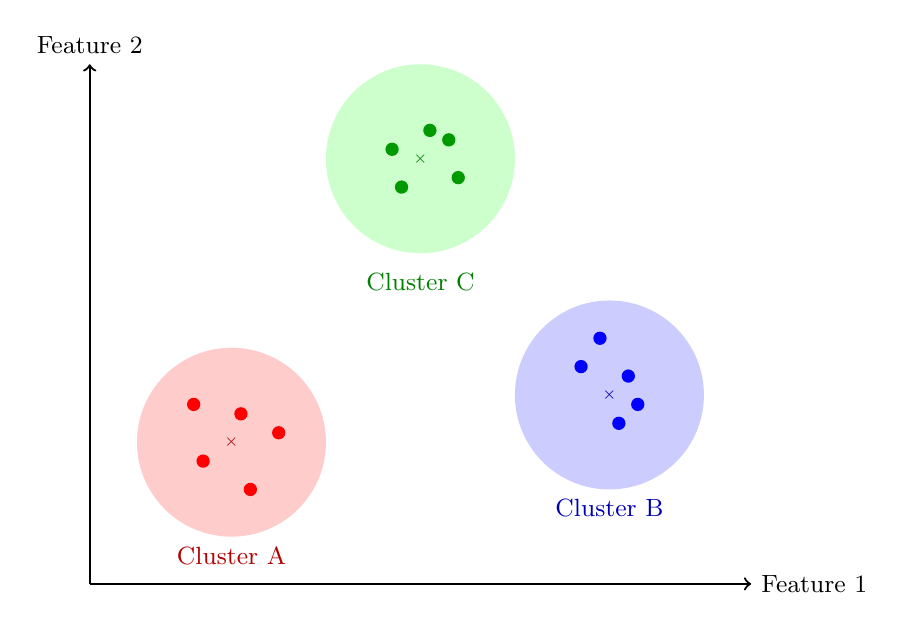
\begin{tikzpicture}[scale=1.2]
		
		% Cluster A - Red
		\fill[red!20] (0,0) circle (1);
		\foreach \x/\y in {0.1/0.3, -0.3/-0.2, 0.2/-0.5, -0.4/0.4, 0.5/0.1} {
			\fill[red] (\x,\y) circle (2pt);
		}
		\node[red!70!black] at (0, -1.2) {\small Cluster A};
		\node[red!70!black] at (0, 0) {\tiny $\times$};
		
		% Cluster B - Blue
		\fill[blue!20] (4,0.5) circle (1);
		\foreach \x/\y in {3.7/0.8, 4.1/0.2, 4.2/0.7, 3.9/1.1, 4.3/0.4} {
			\fill[blue] (\x,\y) circle (2pt);
		}
		\node[blue!70!black] at (4, -0.7) {\small Cluster B};
		\node[blue!70!black] at (4, 0.5) {\tiny $\times$};
		
		% Cluster C - Green
		\fill[green!20] (2,3) circle (1);
		\foreach \x/\y in {1.8/2.7, 2.3/3.2, 2.1/3.3, 1.7/3.1, 2.4/2.8} {
			\fill[green!60!black] (\x,\y) circle (2pt);
		}
		\node[green!50!black] at (2, 1.7) {\small Cluster C};
		\node[green!50!black] at (2, 3) {\tiny $\times$};
		
		% Axes
		\draw[->, thick] (-1.5, -1.5) -- (5.5, -1.5) node[right] {\small Feature 1};
		\draw[->, thick] (-1.5, -1.5) -- (-1.5, 4) node[above] {\small Feature 2};
		
	\end{tikzpicture}
	\caption{Illustration of clustering in 2D feature space with three distinct groups and centroids}
	\label{fig:clustering-tikz}
\end{figure}

\textbf{Clustering} merupakan salah satu teknik utama dalam unsupervised learning yang bertujuan untuk mengelompokkan data ke dalam grup atau klaster berdasarkan kemiripan (similarity) antar data (Gambar~\ref{fig:clustering-tikz}). Dalam clustering, tidak tersedia label atau kategori sebelumnya. Oleh karena itu, algoritma clustering akan secara otomatis mencari pola dan struktur tersembunyi dalam data untuk membentuk grup-grup yang saling homogen di dalam dan heterogen antar kelompok \cite{kelleher2015fundamentals}.

\subsection*{Tujuan Clustering dalam Bisnis}

Dalam konteks bisnis, clustering sangat bermanfaat untuk mendukung pengambilan keputusan berbasis segmentasi, terutama ketika organisasi tidak memiliki label eksplisit terhadap entitas dalam datanya. Beberapa tujuan utama penggunaan clustering dalam dunia bisnis antara lain:

\begin{itemize}
	\item \textbf{Segmentasi pelanggan:} mengelompokkan pelanggan berdasarkan perilaku pembelian, pola interaksi, nilai transaksi, atau demografi untuk menyusun strategi pemasaran yang lebih tepat sasaran.
	\item \textbf{Personalisasi layanan:} menyusun paket produk atau promosi yang disesuaikan dengan profil segmen pelanggan tertentu.
	\item \textbf{Identifikasi pola pemakaian produk:} mengenali kelompok pengguna berdasarkan cara mereka menggunakan layanan atau fitur tertentu.
	\item \textbf{Analisis lokasi:} mengelompokkan wilayah geografis berdasarkan potensi pasar, tingkat permintaan, atau pola distribusi.
\end{itemize}

Dengan melakukan segmentasi otomatis melalui clustering, organisasi dapat meningkatkan efisiensi kampanye pemasaran, meningkatkan kepuasan pelanggan, dan mendukung pengambilan keputusan yang berbasis data.

\subsection*{Metode Clustering Populer}

Terdapat berbagai algoritma clustering yang umum digunakan, masing-masing memiliki pendekatan berbeda dalam mengelompokkan data. Berikut adalah tiga metode yang paling banyak digunakan dalam praktik bisnis:

\paragraph{1. K-Means Clustering.} K-Means adalah algoritma clustering yang membagi data ke dalam \( k \) kelompok berdasarkan jarak rata-rata terhadap pusat klaster (\textit{centroid}). Prosesnya iteratif:
\begin{enumerate}
	\item Tentukan jumlah klaster \( k \),
	\item Inisialisasi pusat klaster secara acak,
	\item Kelompokkan setiap data ke klaster terdekat,
	\item Hitung ulang posisi pusat klaster berdasarkan data yang tergabung,
	\item Ulangi proses hingga konvergen (perubahan posisi klaster minimal).
\end{enumerate}

\textbf{Kelebihan:} cepat, sederhana, cocok untuk data besar.  
\textbf{Kekurangan:} perlu menentukan \( k \) di awal, sensitif terhadap outlier, hanya efektif untuk klaster berbentuk bulat dan ukuran seimbang.

\paragraph{2. Hierarchical Clustering.} Hierarchical clustering membentuk struktur pohon (\textit{dendrogram}) dari data dengan dua pendekatan:
\begin{itemize}
	\item \textbf{Agglomerative (bottom-up):} setiap data dianggap sebagai klaster tunggal, lalu digabung bertahap hingga menjadi satu klaster besar.
	\item \textbf{Divisive (top-down):} mulai dari satu klaster besar, lalu dipisah menjadi klaster lebih kecil secara bertahap.
\end{itemize}

\textbf{Kelebihan:} tidak perlu menentukan jumlah klaster di awal, hasil dapat divisualisasikan secara hierarkis.  
\textbf{Kekurangan:} tidak efisien untuk data besar, sulit diperbarui jika ada data baru.

\paragraph{3. DBSCAN (Density-Based Spatial Clustering of Applications with Noise).} DBSCAN mengelompokkan data berdasarkan kepadatan (density). Dua poin dianggap berada dalam satu klaster jika cukup berdekatan dan terdapat cukup banyak tetangga di sekitarnya. Algoritma ini mampu mendeteksi:
\begin{itemize}
	\item Klaster dengan bentuk arbitrer (tidak harus bulat),
	\item Titik data yang tidak termasuk klaster manapun (anomali atau noise).
\end{itemize}

\textbf{Kelebihan:} tidak perlu menentukan jumlah klaster, mampu menangani bentuk klaster yang kompleks dan mendeteksi outlier.  
\textbf{Kekurangan:} performa menurun pada data berdimensi tinggi, sensitif terhadap parameter jarak dan minimum tetangga.

\subsection*{Pemilihan Metode Clustering}

Pemilihan algoritma clustering bergantung pada:
\begin{itemize}
	\item Bentuk dan ukuran klaster yang diharapkan,
	\item Skala dan dimensi data,
	\item Tujuan analisis (misalnya segmentasi vs. deteksi anomali),
	\item Kebutuhan interpretabilitas dan visualisasi.
\end{itemize}

Dalam praktik bisnis, K-Means sering menjadi pilihan awal karena sederhana dan efisien, sedangkan DBSCAN cocok untuk mendeteksi perilaku ekstrem atau segmen kecil yang tersembunyi. Hierarchical clustering berguna dalam eksplorasi awal untuk memahami struktur segmentasi sebelum menentukan jumlah klaster yang tepat.


\section{Visualisasi dan Reduksi Dimensi}

Dalam dunia bisnis dan analitik data, sering kali kita dihadapkan pada dataset berdimensi tinggi, yaitu data dengan banyak variabel atau fitur. Contohnya adalah data pelanggan dengan ratusan atribut seperti perilaku pembelian, histori transaksi, demografi, dan interaksi digital. Dataset berdimensi tinggi dapat menyulitkan proses analisis, visualisasi, dan pembelajaran mesin. Oleh karena itu, dibutuhkan teknik \textbf{reduksi dimensi} (\textit{dimensionality reduction}) untuk menyederhanakan representasi data tanpa kehilangan informasi penting secara signifikan \cite{kelleher2015fundamentals}.

\subsection*{Mengapa Reduksi Dimensi Penting?}

Reduksi dimensi memiliki beberapa tujuan strategis dalam proses analisis data dan penerapan machine learning:

\begin{itemize}
	\item \textbf{Visualisasi:} Data berdimensi tinggi tidak dapat langsung divisualisasikan. Reduksi dimensi memungkinkan kita memetakan data ke dalam 2 atau 3 dimensi sehingga pola atau kelompok dalam data menjadi terlihat.
	
	\item \textbf{Reduksi noise:} Banyak variabel dalam data dapat mengandung noise (gangguan acak) atau redundansi (informasi berulang). Reduksi dimensi membantu menghilangkan fitur yang tidak relevan atau terlalu berkorelasi.
	
	\item \textbf{Efisiensi komputasi:} Semakin banyak fitur, semakin besar pula beban komputasi dalam pelatihan model machine learning. Reduksi dimensi mempercepat proses ini tanpa mengorbankan performa.
	
	\item \textbf{Mengatasi curse of dimensionality:} Dalam dataset berdimensi tinggi, jarak antar data menjadi kurang bermakna dan model sulit menemukan pola. Reduksi dimensi membantu menghindari fenomena ini.
\end{itemize}

\subsection*{Teknik Populer untuk Reduksi Dimensi}

Beberapa metode telah dikembangkan untuk mereduksi dimensi data. Berikut dua teknik yang paling populer dan banyak digunakan dalam analisis bisnis:

\paragraph{1. Principal Component Analysis (PCA)}

\textbf{PCA} adalah metode linier yang mengubah data asli ke dalam himpunan variabel baru yang disebut \textit{principal components}. Komponen ini merupakan kombinasi linier dari fitur-fitur asli dan disusun berdasarkan kontribusinya terhadap variasi data. Komponen pertama menjelaskan variasi terbesar, diikuti oleh komponen kedua, dan seterusnya.

\textbf{Kelebihan:}
\begin{itemize}
	\item Efisien secara komputasi,
	\item Mudah diinterpretasikan,
	\item Cocok untuk data numerik dan linier.
\end{itemize}

\textbf{Kekurangan:}
\begin{itemize}
	\item Tidak mampu menangkap pola non-linier,
	\item Hasil reduksi sulit dipetakan kembali ke fitur asli.
\end{itemize}

\textbf{Contoh bisnis:} PCA dapat digunakan untuk menyederhanakan data survei pelanggan dengan banyak pertanyaan menjadi beberapa dimensi utama seperti “kepuasan layanan”, “harga”, dan “kualitas produk”.

\paragraph{2. t-Distributed Stochastic Neighbor Embedding (t-SNE)}

\textbf{t-SNE} adalah metode non-linier yang sangat populer untuk \textbf{visualisasi data}. Teknik ini memetakan data berdimensi tinggi ke dalam dua atau tiga dimensi dengan mempertahankan hubungan lokal antar data — artinya, data yang serupa akan dipetakan berdekatan di ruang 2D/3D.

\textbf{Kelebihan:}
\begin{itemize}
	\item Sangat efektif untuk visualisasi klaster atau segmen,
	\item Mampu menangkap struktur kompleks yang tidak linier.
\end{itemize}

\textbf{Kekurangan:}
\begin{itemize}
	\item Tidak cocok untuk pemrosesan data skala besar (mahal secara komputasi),
	\item Tidak cocok sebagai tahap preprocessing sebelum supervised learning,
	\item Hasil visual tidak selalu konsisten jika dijalankan ulang.
\end{itemize}

\textbf{Contoh bisnis:} t-SNE banyak digunakan untuk memvisualisasikan hasil segmentasi pelanggan, sehingga manajer dapat memahami secara intuitif pengelompokan dan relasi antar kelompok pelanggan.

\subsection*{Perbandingan Singkat PCA dan t-SNE}

\begin{center}
	\begin{tabular}{|l|c|c|}
		\hline
		\textbf{Kriteria} & \textbf{PCA} & \textbf{t-SNE} \\
		\hline
		Jenis Algoritma & Linier & Non-linier \\
		Tujuan utama & Reduksi dimensi & Visualisasi klaster \\
		Output utama & Komponen utama & Peta 2D atau 3D \\
		Skalabilitas & Tinggi & Terbatas \\
		Hasil dapat direproduksi & Ya & Tidak selalu \\
		Dapat digunakan untuk training model & Ya & Tidak disarankan \\
		\hline
	\end{tabular}
\end{center}


Reduksi dimensi adalah langkah penting dalam proses analisis data modern, terutama dalam unsupervised learning. Teknik seperti PCA dan t-SNE tidak hanya membantu dalam visualisasi hasil segmentasi, tetapi juga meningkatkan efisiensi dan efektivitas dalam pemrosesan data besar. Dalam konteks bisnis, penggunaan reduksi dimensi memungkinkan pengambil keputusan untuk lebih cepat memahami struktur data yang kompleks dan membentuk strategi yang lebih tajam berdasarkan representasi visual dan analitis yang disederhanakan.


\section{Penerapan Clustering untuk Segmentasi Pelanggan}

Segmentasi pelanggan adalah salah satu penerapan paling umum dari teknik \textit{clustering} dalam dunia bisnis. Tujuan utamanya adalah membagi pelanggan ke dalam beberapa kelompok atau segmen berdasarkan kesamaan karakteristik atau perilaku, sehingga strategi pemasaran dan layanan dapat disesuaikan dengan kebutuhan spesifik tiap kelompok \cite{williams2020data}.

Pendekatan ini sangat berguna bagi perusahaan yang memiliki basis pelanggan besar dan heterogen, di mana perlakuan seragam terhadap semua pelanggan sering kali tidak efektif. Dengan mengenali kelompok pelanggan secara otomatis melalui clustering, perusahaan dapat mengembangkan strategi yang lebih personal, relevan, dan efisien.

\subsection*{Studi Kasus: Segmentasi Pelanggan Toko Online}

Dalam contoh ini, sebuah toko online ingin memahami segmentasi pelanggannya berdasarkan data transaksi historis. Dataset yang digunakan mencakup ribuan pelanggan dan mencatat informasi seperti:

\begin{itemize}
	\item \textbf{Frekuensi pembelian:} jumlah transaksi dalam periode tertentu.
	\item \textbf{Monetary value:} total nilai transaksi (dalam satuan mata uang).
	\item \textbf{Recency:} jumlah hari sejak transaksi terakhir.
	\item \textbf{Kategori produk:} ragam jenis produk yang dibeli.
	\item \textbf{Metode pembayaran:} misalnya transfer, kartu kredit, e-wallet.
\end{itemize}

Untuk analisis awal, dilakukan pemilihan fitur utama menggunakan pendekatan RFM (Recency, Frequency, Monetary) karena telah terbukti efektif dalam analisis perilaku pelanggan. Data kemudian dinormalisasi untuk menghindari bias terhadap fitur dengan skala besar.

\subsection*{Proses Clustering dan Hasilnya}

Setelah data siap, dilakukan \textbf{K-Means Clustering} dengan asumsi awal \( k = 4 \) klaster. Jumlah klaster ditentukan menggunakan metode \textit{elbow} untuk memastikan keseimbangan antara kompleksitas dan akurasi pengelompokan.

\textbf{Hasil clustering} menunjukkan empat kelompok pelanggan utama sebagai berikut:

\begin{enumerate}
	\item \textbf{Klaster A – Pelanggan Loyal:} frekuensi tinggi, nilai transaksi tinggi, dan recency rendah. Segmen ini adalah pelanggan paling aktif dan setia. Cocok untuk program loyalitas atau VIP.
	
	\item \textbf{Klaster B – Pelanggan Potensial:} frekuensi dan nilai transaksi sedang, namun dengan recency rendah. Mereka baru-baru ini bertransaksi, sehingga berpotensi dikembangkan menjadi pelanggan loyal.
	
	\item \textbf{Klaster C – Pelanggan Pasif:} frekuensi rendah, nilai transaksi rendah, dan recency tinggi. Mereka jarang melakukan pembelian dan terakhir bertransaksi sudah lama. Strategi reaktivasi dapat digunakan untuk segmen ini.
	
	\item \textbf{Klaster D – Pelanggan Sensitif Harga:} frekuensi cukup sering namun dengan nilai transaksi rendah. Mereka cenderung melakukan pembelian kecil dan mungkin hanya tertarik pada promosi. Cocok untuk kampanye diskon atau bundling.
\end{enumerate}

\subsection*{Manfaat Bisnis dari Segmentasi}

Dengan hasil klaster di atas, perusahaan dapat menyusun strategi yang lebih terfokus:

\begin{itemize}
	\item Menawarkan \textbf{insentif eksklusif} bagi pelanggan loyal untuk menjaga retensi.
	\item Mengembangkan \textbf{email campaign bertarget} untuk mengajak pelanggan pasif kembali.
	\item Merancang \textbf{paket diskon atau promo} untuk pelanggan sensitif harga.
	\item Meluncurkan \textbf{program onboarding} bagi pelanggan baru dalam klaster potensial.
\end{itemize}

Pendekatan ini juga membantu dalam alokasi anggaran pemasaran secara lebih efisien, karena setiap segmen memiliki kebutuhan dan perilaku yang berbeda. Selain itu, hasil clustering dapat digunakan sebagai masukan dalam sistem rekomendasi, analisis churn, dan strategi penetapan harga.

\subsection*{Visualisasi dan Evaluasi}

Setelah klaster terbentuk, visualisasi menggunakan \textbf{PCA} atau \textbf{t-SNE} dapat dilakukan untuk memetakan pelanggan dalam ruang dua dimensi. Hal ini memudahkan manajer untuk melihat distribusi dan kedekatan antar klaster. Warna yang berbeda dapat digunakan untuk menandai klaster, dan ciri khas tiap kelompok dapat dianalisis dengan melihat distribusi fitur utama di masing-masing segmen.

Meskipun clustering adalah metode eksploratif, evaluasi dapat dilakukan dengan menggunakan \textbf{silhouette score} atau \textbf{Davies-Bouldin Index} untuk mengukur seberapa baik pemisahan antar klaster dan kepadatan dalam klaster.

Melalui penerapan clustering untuk segmentasi pelanggan, perusahaan dapat lebih memahami perilaku konsumennya dan membangun strategi yang tidak hanya berdasarkan intuisi, tetapi juga berdasarkan struktur data yang konkret dan terukur.


\section{Hands-On Orange: Segmentasi Pelanggan dengan K-Means}

Orange adalah perangkat lunak visualisasi dan analisis data berbasis komponen yang sangat cocok untuk pembelajaran konsep machine learning secara praktis dan intuitif. Salah satu keunggulan Orange adalah kemampuannya untuk membangun alur kerja (\textit{workflow}) melalui antarmuka drag-and-drop, tanpa perlu menulis kode. Pada bagian ini, akan dijelaskan langkah-langkah praktis untuk menerapkan \textbf{K-Means Clustering} dalam kasus segmentasi pelanggan menggunakan Orange.

\subsection*{Tujuan Praktikum}

Tujuan dari sesi hands-on ini adalah untuk membagi pelanggan ke dalam beberapa segmen berdasarkan perilaku atau atribut tertentu, menggunakan algoritma K-Means. Setelah segmentasi berhasil dilakukan, hasilnya akan divisualisasikan dan dianalisis untuk melihat pola kelompok yang terbentuk.

\subsection*{Dataset}

Untuk praktikum ini digunakan dataset pelanggan dalam format CSV (Comma Separated Values) dengan beberapa fitur utama, antara lain:

\begin{itemize}
	\item \textbf{Recency}: jumlah hari sejak transaksi terakhir.
	\item \textbf{Frequency}: jumlah transaksi yang dilakukan.
	\item \textbf{Monetary}: total nilai pembelian.
	\item \textbf{Customer ID}: identifikasi unik pelanggan (tidak digunakan untuk clustering).
\end{itemize}

Dataset ini tersedia secara publik dan dapat diunduh melalui tautan berikut:

\begin{itemize}
	\item \textbf{UCI Machine Learning Repository}: \url{https://archive.ics.uci.edu/ml/datasets/Online+Retail}
	\item \textbf{Versi RFM siap pakai/}:\\ \url{https://u.pcloud.link/publink/show?code=kZ6a7W5Zr4Y3H3bMCSfxrMGxSut20VEohrGk} dengan nama file \texttt{frm\_results.csv}.
\texttt{}\end{itemize}

Pastikan dataset sudah tersedia secara lokal sebelum memulai proses dan disimpan dalam format \texttt{.csv} agar dapat langsung dibaca oleh komponen \texttt{File} di Orange.


\subsection*{Langkah-langkah Penyusunan Workflow}

\begin{figure}[h]
	\centering
	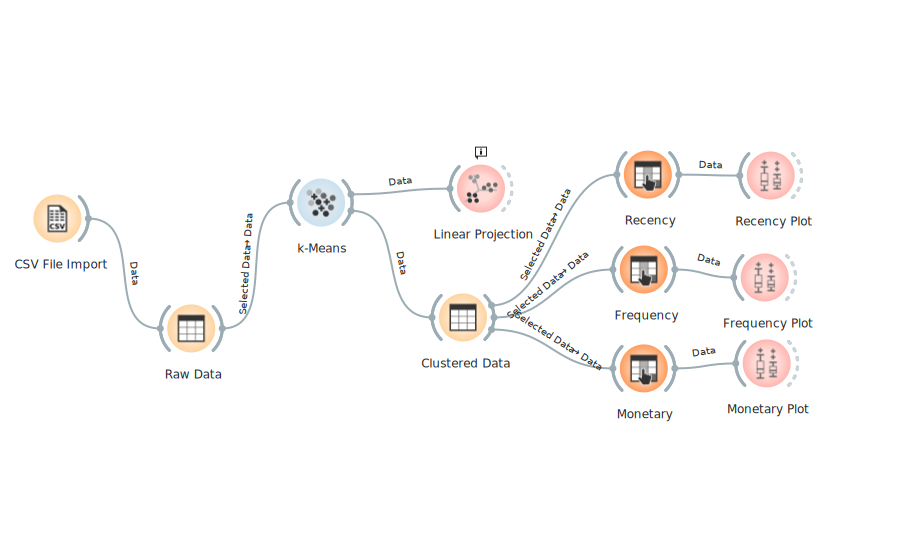
\includegraphics[width=\linewidth]{../figures/clustering.png}
	\caption{Segmentasi pelanggan menggunakan algoritma clustering K-Means}
	\label{fig:clustering-orange}
\end{figure}

Gambar \ref{fig:clustering-orange} menunjukkan alur lengkap untuk melakukan segmentasi pelanggan dengan algoritma K-Means di Orange. Langkah-langkah penyusunan workflow adalah sebagai berikut:

\begin{enumerate}
	\item \textbf{CSV File Import}: Mulai dengan mengimpor dataset menggunakan widget \texttt{File}, lalu arahkan ke file \texttt{frm\_results.csv}.
	\item \textbf{Raw Data}: Data mentah yang diimpor akan ditampilkan pada widget \texttt{Data Table} untuk verifikasi dan pemilihan fitur.
	\item \textbf{k-Means}: Hubungkan data ke widget \texttt{k-Means} untuk melakukan proses clustering. Pilih jumlah klaster yang diinginkan (misalnya 3).
	\item \textbf{Clustered Data}: Output dari \texttt{k-Means} akan diteruskan ke widget \texttt{Data Table} untuk melihat hasil klasterisasi.
	\item \textbf{Linear Projection}: Gunakan \texttt{Linear Projection} untuk memvisualisasikan hasil clustering dalam bentuk dua dimensi (scatter plot).
	\item \textbf{Cluster Statistics}: Bagi hasil klaster menjadi beberapa subset (misalnya \texttt{Cluster 1}, \texttt{Cluster 2}, \texttt{Cluster 3}), kemudian analisis masing-masing menggunakan widget \texttt{Statistics}.
	\item \textbf{RFM Plotting}: Pisahkan data berdasarkan atribut \texttt{Recency}, \texttt{Frequency}, dan \texttt{Monetary}, kemudian gunakan widget \texttt{Box Plot} untuk masing-masing atribut guna memahami distribusi nilai dalam tiap klaster.
\end{enumerate}

\begin{figure}[h]
	\centering
	\begin{subfigure}[t]{0.48\textwidth}
		\centering
		\fbox{\includegraphics[width=\linewidth]{../figures/3d_plot.png}}
		\caption{Cluster in 3D (RFM space)}
	\end{subfigure}
	\hfill
	\begin{subfigure}[t]{0.48\textwidth}
		\centering
		\fbox{\includegraphics[width=\linewidth]{../figures/recency.png}}
		\caption{Recency Distribution}
	\end{subfigure}
	
	\vspace{10pt}
	
	\begin{subfigure}[t]{0.48\textwidth}
		\centering
		\fbox{\includegraphics[width=\linewidth]{../figures/frequency.png}}
		\caption{Frequency Distribution}
	\end{subfigure}
	\hfill
	\begin{subfigure}[t]{0.48\textwidth}
		\centering
		\fbox{\includegraphics[width=\linewidth]{../figures/monetary.png}}
		\caption{Monetary Distribution}
	\end{subfigure}
	
	\caption{Customer segmentation results using K-Means: cluster layout and RFM distribution}
	\label{fig:clustering-subfigures}
\end{figure}


\subsection*{Analisis Hasil}

Setelah workflow selesai, hasil clustering dapat dianalisis sebagai berikut:

\begin{itemize}
	\item Amati ukuran masing-masing klaster (jumlah pelanggan dalam tiap segmen).
	\item Identifikasi karakteristik khas setiap klaster, misalnya:
	\begin{itemize}
		\item Klaster dengan \texttt{Monetary} tinggi $\rightarrow$ pelanggan VIP.
		\item Klaster dengan \texttt{Recency} tinggi dan \texttt{Frequency} rendah $\rightarrow$ pelanggan pasif.
	\end{itemize}
	\item Gunakan hasil ini untuk menyusun strategi pemasaran berbeda bagi tiap segmen.
\end{itemize}

Melalui workflow sederhana di Orange, proses segmentasi pelanggan dapat dilakukan tanpa menulis kode. Penggunaan K-Means sebagai metode clustering memperlihatkan bagaimana pelanggan dapat dikelompokkan berdasarkan perilaku belanja mereka. Visualisasi hasil dalam \textit{scatter plot} juga membantu memahami struktur kelompok yang terbentuk secara intuitif. Praktikum ini memberi dasar penting untuk memahami penerapan unsupervised learning dalam pengambilan keputusan bisnis.


\section{Interpretasi Hasil Segmentasi dan Strategi Bisnis}

Setelah proses segmentasi pelanggan menggunakan algoritma K-Means, diperoleh tiga klaster yang berbeda berdasarkan atribut Recency, Frequency, dan Monetary (RFM). Interpretasi dari masing-masing klaster sangat penting untuk merancang strategi bisnis yang lebih tepat sasaran dan berbasis data.

\subsection{Profil Klaster dan Pemberian Label}

\textbf{Klaster C1 – \textit{Dormant Buyers}} (Pelanggan Tidak Aktif):  
Kelompok ini ditandai dengan nilai recency yang sangat tinggi (rata-rata 246 hari), frekuensi pembelian yang sangat rendah (1,58 kali), serta nilai transaksi yang juga sangat kecil (sekitar 629). Pelanggan dalam klaster ini sudah lama tidak bertransaksi dan memiliki tingkat keterlibatan yang sangat rendah. Mereka berisiko tinggi untuk churn dan memerlukan pendekatan reaktivasi.

\textbf{Klaster C2 – \textit{Regular Shoppers}} (Pelanggan Reguler):  
Pelanggan dalam klaster ini memiliki recency sedang (sekitar 41 hari), frekuensi pembelian sedang (4,68 kali), dan nilai transaksi yang moderat (sekitar 1.859). Mereka menunjukkan perilaku yang konsisten, namun belum tergolong bernilai tinggi. Klaster ini berpotensi dikembangkan lebih lanjut melalui strategi upselling dan peningkatan loyalitas.

\textbf{Klaster C3 – \textit{VIP Customers}} (Pelanggan Sangat Aktif dan Bernilai Tinggi):  
Klaster ini mencakup pelanggan terbaik dengan recency sangat rendah (rata-rata 6 hari), frekuensi transaksi yang tinggi (66,5 kali), dan nilai pembelanjaan yang sangat besar (sekitar 85.900). Mereka sangat aktif dan memberikan kontribusi signifikan terhadap pendapatan. Retensi dan pemeliharaan relasi dengan segmen ini menjadi prioritas utama.

\subsection{Implikasi Strategis}

Setiap label klaster mewakili segmen dengan perilaku dan kebutuhan berbeda. Oleh karena itu, strategi pemasaran harus disesuaikan.

Untuk \textit{VIP Customers}, fokus utama adalah mempertahankan loyalitas dengan pendekatan personal, seperti pemberian hadiah eksklusif, penawaran prioritas, atau akses awal ke produk baru. Hal ini memperkuat hubungan emosional dan memastikan retensi jangka panjang.

\textit{Regular Shoppers} perlu didorong agar naik kelas menjadi pelanggan bernilai tinggi. Strategi seperti diskon bundling, program loyalitas berbasis poin, atau promosi terbatas dapat meningkatkan frekuensi dan nilai transaksi mereka.

Sementara itu, \textit{Dormant Buyers} membutuhkan pendekatan pemulihan. Kampanye “kita rindu Anda,” penawaran spesial untuk kembali bertransaksi, atau survei kepuasan untuk mengetahui alasan ketidakterlibatan dapat membantu mengaktifkan kembali segmen ini.

\subsection{Arah Kebijakan Retensi dan Pemasaran Berbasis Segmen}

Dengan label yang jelas, masing-masing klaster dapat dipetakan dalam strategi retensi dan alokasi anggaran pemasaran secara lebih efisien. Upaya pemasaran bernilai tinggi bisa difokuskan pada \textit{VIP Customers}, sedangkan automasi email atau penawaran massal digunakan untuk segmen \textit{Dormant Buyers}.

Segmentasi juga membantu pemantauan performa tiap segmen secara berkala—misalnya, dengan mengukur tingkat retensi, repeat purchase, dan lifetime value per klaster. Data ini menjadi dasar untuk mengukur keberhasilan strategi dan melakukan penyesuaian secara dinamis.

Dengan memahami siapa pelanggan terbaik, siapa yang konsisten namun bisa ditingkatkan, dan siapa yang mulai tidak aktif, perusahaan dapat mengambil keputusan bisnis yang lebih tepat, berbasis data, dan berdampak langsung terhadap pertumbuhan jangka panjang.


%\section{Anomali Deteksi untuk Pencegahan Risiko}
%% Deteksi anomali sebagai bagian dari unsupervised learning.
%% Aplikasi dalam fraud detection, outlier detection, dan quality control.
%
%\section{Hands-On Orange: Deteksi Anomali pada Dataset Keuangan}
%% Praktik membangun pipeline deteksi anomali dengan Orange.
%% Contoh: outlier detection pada data transaksi.
%
%\section{Kelebihan, Keterbatasan, dan Tantangan Unsupervised Learning}
%% Keuntungan eksploratif, tidak butuh label.
%% Tantangan: interpretasi, validasi hasil, sensitivitas parameter.

\section{Rangkuman}

Unsupervised learning memainkan peran penting dalam konteks \textit{Big Data for Business} karena mampu mengungkap pola tersembunyi dalam data tanpa memerlukan label atau anotasi sebelumnya. Melalui teknik seperti clustering dan reduksi dimensi, pelaku bisnis dapat memahami struktur data pelanggan, mendeteksi anomali, dan melakukan segmentasi pasar secara otomatis. Pendekatan ini sangat berguna ketika volume data besar dan kompleks, serta ketika label sulit atau mahal untuk diperoleh.

Jika dibandingkan dengan supervised learning yang bergantung pada data berlabel untuk melakukan prediksi atau klasifikasi, unsupervised learning lebih bersifat eksploratif dan digunakan untuk penemuan wawasan baru. Meskipun hasilnya sering kali tidak langsung terverifikasi secara eksplisit, kemampuan unsupervised learning untuk mengekstrak struktur dan relasi dari data menjadikannya komponen esensial dalam strategi analitik bisnis modern.

